% Options for packages loaded elsewhere
\PassOptionsToPackage{unicode}{hyperref}
\PassOptionsToPackage{hyphens}{url}
%
\documentclass[
]{book}
\usepackage{amsmath,amssymb}
\usepackage{lmodern}
\usepackage{ifxetex,ifluatex}
\ifnum 0\ifxetex 1\fi\ifluatex 1\fi=0 % if pdftex
  \usepackage[T1]{fontenc}
  \usepackage[utf8]{inputenc}
  \usepackage{textcomp} % provide euro and other symbols
\else % if luatex or xetex
  \usepackage{unicode-math}
  \defaultfontfeatures{Scale=MatchLowercase}
  \defaultfontfeatures[\rmfamily]{Ligatures=TeX,Scale=1}
\fi
% Use upquote if available, for straight quotes in verbatim environments
\IfFileExists{upquote.sty}{\usepackage{upquote}}{}
\IfFileExists{microtype.sty}{% use microtype if available
  \usepackage[]{microtype}
  \UseMicrotypeSet[protrusion]{basicmath} % disable protrusion for tt fonts
}{}
\makeatletter
\@ifundefined{KOMAClassName}{% if non-KOMA class
  \IfFileExists{parskip.sty}{%
    \usepackage{parskip}
  }{% else
    \setlength{\parindent}{0pt}
    \setlength{\parskip}{6pt plus 2pt minus 1pt}}
}{% if KOMA class
  \KOMAoptions{parskip=half}}
\makeatother
\usepackage{xcolor}
\IfFileExists{xurl.sty}{\usepackage{xurl}}{} % add URL line breaks if available
\IfFileExists{bookmark.sty}{\usepackage{bookmark}}{\usepackage{hyperref}}
\hypersetup{
  pdftitle={Statisztika könyvek},
  pdfauthor={Abari Kálmán},
  hidelinks,
  pdfcreator={LaTeX via pandoc}}
\urlstyle{same} % disable monospaced font for URLs
\usepackage{color}
\usepackage{fancyvrb}
\newcommand{\VerbBar}{|}
\newcommand{\VERB}{\Verb[commandchars=\\\{\}]}
\DefineVerbatimEnvironment{Highlighting}{Verbatim}{commandchars=\\\{\}}
% Add ',fontsize=\small' for more characters per line
\usepackage{framed}
\definecolor{shadecolor}{RGB}{248,248,248}
\newenvironment{Shaded}{\begin{snugshade}}{\end{snugshade}}
\newcommand{\AlertTok}[1]{\textcolor[rgb]{0.94,0.16,0.16}{#1}}
\newcommand{\AnnotationTok}[1]{\textcolor[rgb]{0.56,0.35,0.01}{\textbf{\textit{#1}}}}
\newcommand{\AttributeTok}[1]{\textcolor[rgb]{0.77,0.63,0.00}{#1}}
\newcommand{\BaseNTok}[1]{\textcolor[rgb]{0.00,0.00,0.81}{#1}}
\newcommand{\BuiltInTok}[1]{#1}
\newcommand{\CharTok}[1]{\textcolor[rgb]{0.31,0.60,0.02}{#1}}
\newcommand{\CommentTok}[1]{\textcolor[rgb]{0.56,0.35,0.01}{\textit{#1}}}
\newcommand{\CommentVarTok}[1]{\textcolor[rgb]{0.56,0.35,0.01}{\textbf{\textit{#1}}}}
\newcommand{\ConstantTok}[1]{\textcolor[rgb]{0.00,0.00,0.00}{#1}}
\newcommand{\ControlFlowTok}[1]{\textcolor[rgb]{0.13,0.29,0.53}{\textbf{#1}}}
\newcommand{\DataTypeTok}[1]{\textcolor[rgb]{0.13,0.29,0.53}{#1}}
\newcommand{\DecValTok}[1]{\textcolor[rgb]{0.00,0.00,0.81}{#1}}
\newcommand{\DocumentationTok}[1]{\textcolor[rgb]{0.56,0.35,0.01}{\textbf{\textit{#1}}}}
\newcommand{\ErrorTok}[1]{\textcolor[rgb]{0.64,0.00,0.00}{\textbf{#1}}}
\newcommand{\ExtensionTok}[1]{#1}
\newcommand{\FloatTok}[1]{\textcolor[rgb]{0.00,0.00,0.81}{#1}}
\newcommand{\FunctionTok}[1]{\textcolor[rgb]{0.00,0.00,0.00}{#1}}
\newcommand{\ImportTok}[1]{#1}
\newcommand{\InformationTok}[1]{\textcolor[rgb]{0.56,0.35,0.01}{\textbf{\textit{#1}}}}
\newcommand{\KeywordTok}[1]{\textcolor[rgb]{0.13,0.29,0.53}{\textbf{#1}}}
\newcommand{\NormalTok}[1]{#1}
\newcommand{\OperatorTok}[1]{\textcolor[rgb]{0.81,0.36,0.00}{\textbf{#1}}}
\newcommand{\OtherTok}[1]{\textcolor[rgb]{0.56,0.35,0.01}{#1}}
\newcommand{\PreprocessorTok}[1]{\textcolor[rgb]{0.56,0.35,0.01}{\textit{#1}}}
\newcommand{\RegionMarkerTok}[1]{#1}
\newcommand{\SpecialCharTok}[1]{\textcolor[rgb]{0.00,0.00,0.00}{#1}}
\newcommand{\SpecialStringTok}[1]{\textcolor[rgb]{0.31,0.60,0.02}{#1}}
\newcommand{\StringTok}[1]{\textcolor[rgb]{0.31,0.60,0.02}{#1}}
\newcommand{\VariableTok}[1]{\textcolor[rgb]{0.00,0.00,0.00}{#1}}
\newcommand{\VerbatimStringTok}[1]{\textcolor[rgb]{0.31,0.60,0.02}{#1}}
\newcommand{\WarningTok}[1]{\textcolor[rgb]{0.56,0.35,0.01}{\textbf{\textit{#1}}}}
\usepackage{longtable,booktabs,array}
\usepackage{calc} % for calculating minipage widths
% Correct order of tables after \paragraph or \subparagraph
\usepackage{etoolbox}
\makeatletter
\patchcmd\longtable{\par}{\if@noskipsec\mbox{}\fi\par}{}{}
\makeatother
% Allow footnotes in longtable head/foot
\IfFileExists{footnotehyper.sty}{\usepackage{footnotehyper}}{\usepackage{footnote}}
\makesavenoteenv{longtable}
\usepackage{graphicx}
\makeatletter
\def\maxwidth{\ifdim\Gin@nat@width>\linewidth\linewidth\else\Gin@nat@width\fi}
\def\maxheight{\ifdim\Gin@nat@height>\textheight\textheight\else\Gin@nat@height\fi}
\makeatother
% Scale images if necessary, so that they will not overflow the page
% margins by default, and it is still possible to overwrite the defaults
% using explicit options in \includegraphics[width, height, ...]{}
\setkeys{Gin}{width=\maxwidth,height=\maxheight,keepaspectratio}
% Set default figure placement to htbp
\makeatletter
\def\fps@figure{htbp}
\makeatother
\setlength{\emergencystretch}{3em} % prevent overfull lines
\providecommand{\tightlist}{%
  \setlength{\itemsep}{0pt}\setlength{\parskip}{0pt}}
\setcounter{secnumdepth}{5}
\usepackage{booktabs}
\usepackage{fontspec}
\usepackage{multirow}
\usepackage{multicol}
\usepackage{colortbl}
\usepackage{hhline}
\usepackage{longtable}
\usepackage{array}
\usepackage{hyperref}
\ifluatex
  \usepackage{selnolig}  % disable illegal ligatures
\fi
\usepackage[]{natbib}
\bibliographystyle{apalike}

\title{Statisztika könyvek}
\author{Abari Kálmán}
\date{2021-08-30}

\begin{document}
\maketitle

{
\setcounter{tocdepth}{1}
\tableofcontents
}
\hypertarget{bevezetuxe9s}{%
\chapter{Bevezetés}\label{bevezetuxe9s}}

Jelen jegyzet célja a statisztika tanulmányok segítése. Számos segítő könyv, jegyzet, tutoriál és blog érhető el akár szabadon is az interneten, de a kereskedelmi forgalomban lévő anyagokhoz is számos ingyenesen hozzáférhető adatbázis vagy egyéb kiegészítés létezik. Ezeket a tartalmakat dolgozzuk fel, és tesszük elérhetővé az érdeklődők számára. Könyvünkben megkülönböztetett figyelmet szentelünk a pszichológia témakörének, de más tudományágak anyagai megjelenhetnek itt.

Jelen kötet egy együttműködés keretében jött létre, így számos szerzője van:

\begin{itemize}
\tightlist
\item
  Abari Kálmán
\end{itemize}

\hypertarget{ingyenes-kuxf6nyvek}{%
\chapter{Ingyenes könyvek}\label{ingyenes-kuxf6nyvek}}

\begin{itemize}
\item
  ONLINESTAT - \href{http://onlinestatbook.com/}{A könyv elérése}\\
  Online Statistics Education: A Multimedia Course of Study (\url{http://onlinestatbook.com/}). Project Leader: David M. Lane, Rice University.
\item
  JASPDATA - \href{https://jasp-stats.org/wp-content/uploads/2020/05/The_JASP_Data_Library_1st_Edition.pdf}{A könyv elérése}\\
  Wagenmakers, E.-J., Kucharský, Š., \& the JASP Team. (2020). The JASP Data Library (1st ed.). \url{https://doi.org/10.6084/m9.figshare.9980744}
\end{itemize}

\hypertarget{adatbuxe1zis-puxe9lduxe1k-a-kuxf6nyvekbux151l}{%
\chapter{Adatbázis példák a könyvekből}\label{adatbuxe1zis-puxe9lduxe1k-a-kuxf6nyvekbux151l}}

\hypertarget{onlinestat}{%
\section{ONLINESTAT}\label{onlinestat}}

\textbf{Hivatkozás a könyvre:}

Online Statistics Education: A Multimedia Course of Study (\url{http://onlinestatbook.com/}). Project Leader: David M. Lane, Rice University.

\href{http://onlinestatbook.com/}{A könyv elérése}

\hypertarget{a-leniency-adatbuxe1zis}{%
\subsection{\texorpdfstring{A \texttt{leniency} adatbázis}{A leniency adatbázis}}\label{a-leniency-adatbuxe1zis}}

\hypertarget{leuxedruxe1s}{%
\subsubsection*{Leírás}\label{leuxedruxe1s}}
\addcontentsline{toc}{subsubsection}{Leírás}

A mosoly növeli az engedékenységet? A különböző típusú mosolyok eltérően hatékonyak? Mosolyogjunk ha bajban vagyunk?

Bizonyítékok vannak arra, hogy a mosolygás enyhítheti az esetleges jogsértések megítélését. Ez a ``mosoly-engedékenység'' elnevezésű jelenség volt Marianne LaFrance és Marvin Hecht 1995-ös tanulmányának középpontjában.

A mosoly segít barátokat nyerni és befolyásolni az embereket. A mosolygás hatásaival kapcsolatos kutatások ezt alátámasztották, és kimutatták, hogy a mosolygó embert kellemesebbnek, vonzóbbnak, őszintébbnek, társaságkedvelőbbnek és hozzáértőbbnek ítélik meg, mint a nem mosolygó embert.

A vizsgálatban egy iskolai szabálytalanságot kellett megítélni a vizsgálati személyeknek, melynek leírásához egy fényképet is csatoltak az elkövetőről. A fényképen szereplő személy mosolya 4 kategória egyikébe esik: hamis mosoly, érzelmes mosoly, kényszerült mosoly, semleges ``mosoly''. Az utóbbi neutrális arckifejezés kontrollként került a vizsgálatba. Minden vizsgálati személy pontosan egy feltételben szerepelt. Ez korlátozhatja az eredmények általánosíthatóságát.

\hypertarget{vuxe1ltozuxf3k}{%
\subsubsection*{Változók}\label{vuxe1ltozuxf3k}}
\addcontentsline{toc}{subsubsection}{Változók}

\begin{itemize}
\tightlist
\item
  \texttt{smile} (faktor) - a fényképen szereplő személy mosolya. Lehetséges értékei:

  \begin{itemize}
  \tightlist
  \item
    \texttt{1} - hamis (false smile)
  \item
    \texttt{2} - érzelmes (felt smile)
  \item
    \texttt{3} - kényszerült (miserable smile)
  \item
    \texttt{4} - semleges (neutral control)
  \end{itemize}
\item
  \texttt{leniency} (numerikus) - annak a mértéke, hogy mennyire voltak engedékenyek az ítéletek.
\end{itemize}

\hypertarget{hivatkozuxe1s}{%
\subsubsection*{Hivatkozás}\label{hivatkozuxe1s}}
\addcontentsline{toc}{subsubsection}{Hivatkozás}

\begin{itemize}
\tightlist
\item
  LaFrance, M., \& Hecht, M. A. (1995) Why smiles generate leniency. Personality and Social Psychology Bulletin, 21, 207-214.
\item
  \href{https://onlinestatbook.com/2/case_studies/leniency.html}{Smiles and Leniency}
\item
  \href{https://onlinestatbook.com/2/analysis_of_variance/one-way.html}{One-Factor ANOVA (Between Subjects)}
\end{itemize}

\hypertarget{kapcsoluxf3duxf3-r-sorok}{%
\subsubsection*{Kapcsolódó R sorok}\label{kapcsoluxf3duxf3-r-sorok}}
\addcontentsline{toc}{subsubsection}{Kapcsolódó R sorok}

\begin{Shaded}
\begin{Highlighting}[]
\CommentTok{\# Beolvasás}
\NormalTok{leniency }\OtherTok{\textless{}{-}} \FunctionTok{read.csv}\NormalTok{(}\AttributeTok{file =} \StringTok{"adat/onlinestat/leniency.csv"}\NormalTok{,}
                     \AttributeTok{sep =} \StringTok{","}\NormalTok{, }
                     \AttributeTok{dec =} \StringTok{"."}\NormalTok{,}
                     \AttributeTok{header =}\NormalTok{ T, }
                     \AttributeTok{quote =} \StringTok{""}\NormalTok{,  }
                     \AttributeTok{comment.char =} \StringTok{""}\NormalTok{, }
                     \AttributeTok{fileEncoding =} \StringTok{"UTF{-}8"}
\NormalTok{                    )}
\CommentTok{\# Típuskonverzió}
\NormalTok{leniency}\SpecialCharTok{$}\NormalTok{smile }\OtherTok{\textless{}{-}} \FunctionTok{factor}\NormalTok{(leniency}\SpecialCharTok{$}\NormalTok{smile, }
    \AttributeTok{levels =} \FunctionTok{c}\NormalTok{(}\StringTok{"1"}\NormalTok{, }\StringTok{"2"}\NormalTok{, }\StringTok{"3"}\NormalTok{, }\StringTok{"4"}\NormalTok{),}
    \AttributeTok{labels =} \FunctionTok{c}\NormalTok{(}\StringTok{"hamis"}\NormalTok{, }\StringTok{"érzelmes"}\NormalTok{, }\StringTok{"kényszerült"}\NormalTok{, }\StringTok{"semleges"}\NormalTok{))}

\CommentTok{\# Leíró statisztikai mutatók}
\FunctionTok{library}\NormalTok{(DescTools)}
\FunctionTok{Desc}\NormalTok{(}\AttributeTok{formula =}\NormalTok{ leniency}\SpecialCharTok{\textasciitilde{}}\NormalTok{smile, }\AttributeTok{data =}\NormalTok{ leniency, }\AttributeTok{plotit =}\NormalTok{ F)}
\CommentTok{\#\textgreater{} {-}{-}{-}{-}{-}{-}{-}{-}{-}{-}{-}{-}{-}{-}{-}{-}{-}{-}{-}{-}{-}{-}{-}{-}{-}{-}{-}{-}{-}{-}{-}{-}{-}{-}{-}{-}{-}{-}{-}{-}{-}{-}{-}{-}{-}{-}{-}{-}{-}{-}{-}{-}{-}{-}{-}{-}{-}{-} }
\CommentTok{\#\textgreater{} leniency \textasciitilde{} smile (leniency)}
\CommentTok{\#\textgreater{} }
\CommentTok{\#\textgreater{} Summary: }
\CommentTok{\#\textgreater{} n pairs: 136, valid: 136 (100.0\%), missings: 0 (0.0\%), groups: 4}
\CommentTok{\#\textgreater{} }
\CommentTok{\#\textgreater{}                                                           }
\CommentTok{\#\textgreater{}               hamis     érzelmes  kényszerült     semleges}
\CommentTok{\#\textgreater{} mean          5.368        4.912        4.912        4.118}
\CommentTok{\#\textgreater{} median        5.500        4.750        4.750        4.000}
\CommentTok{\#\textgreater{} sd            1.827        1.681        1.454        1.523}
\CommentTok{\#\textgreater{} IQR           2.875        2.375        1.500        1.875}
\CommentTok{\#\textgreater{} n                34           34           34           34}
\CommentTok{\#\textgreater{} np          25.000\%      25.000\%      25.000\%      25.000\%}
\CommentTok{\#\textgreater{} NAs               0            0            0            0}
\CommentTok{\#\textgreater{} 0s                0            0            0            0}
\CommentTok{\#\textgreater{} }
\CommentTok{\#\textgreater{} Kruskal{-}Wallis rank sum test:}
\CommentTok{\#\textgreater{}   Kruskal{-}Wallis chi{-}squared = 9.1747, df = 3, p{-}value = 0.02706}
\end{Highlighting}
\end{Shaded}

\begin{Shaded}
\begin{Highlighting}[]
\CommentTok{\# Leíró statisztikai mutatók}
\FunctionTok{library}\NormalTok{(summarytools)}
\FunctionTok{st\_options}\NormalTok{(}\StringTok{"headings"}\NormalTok{, }\ConstantTok{FALSE}\NormalTok{)}
\FunctionTok{stby}\NormalTok{(}\AttributeTok{data =}\NormalTok{ leniency}\SpecialCharTok{$}\NormalTok{leniency, }\AttributeTok{INDICES =}\NormalTok{ leniency}\SpecialCharTok{$}\NormalTok{smile, }
    \AttributeTok{FUN =}\NormalTok{ descr,}
    \AttributeTok{stats =} \FunctionTok{c}\NormalTok{(}\StringTok{"n.valid"}\NormalTok{, }\StringTok{"mean"}\NormalTok{, }\StringTok{"med"}\NormalTok{, }\StringTok{"sd"}\NormalTok{, }\StringTok{"iqr"}\NormalTok{),}
    \AttributeTok{transpose =} \ConstantTok{FALSE}\NormalTok{,}
    \AttributeTok{style=}\StringTok{"rmarkdown"}\NormalTok{,}
    \AttributeTok{caption=}\StringTok{"Leíró statisztika"}\NormalTok{) }
\end{Highlighting}
\end{Shaded}

\begin{longtable}[]{@{}lrrrr@{}}
\caption{Leíró statisztika}\tabularnewline
\toprule
& hamis & érzelmes & kényszerült & semleges \\
\midrule
\endfirsthead
\toprule
& hamis & érzelmes & kényszerült & semleges \\
\midrule
\endhead
N.Valid & 34.00 & 34.00 & 34.00 & 34.00 \\
Mean & 5.37 & 4.91 & 4.91 & 4.12 \\
Median & 5.50 & 4.75 & 4.75 & 4.00 \\
Std.Dev & 1.83 & 1.68 & 1.45 & 1.52 \\
IQR & 2.88 & 2.38 & 1.50 & 1.88 \\
\bottomrule
\end{longtable}

\begin{Shaded}
\begin{Highlighting}[]
\CommentTok{\# Ábra {-} dobozdiagram}
\FunctionTok{library}\NormalTok{(ggplot2)}
\FunctionTok{ggplot}\NormalTok{(}\AttributeTok{data =}\NormalTok{ leniency, }\AttributeTok{mapping =} \FunctionTok{aes}\NormalTok{(}\AttributeTok{x=}\NormalTok{smile, }\AttributeTok{y=}\NormalTok{leniency, }\AttributeTok{fill=}\NormalTok{smile)) }\SpecialCharTok{+} 
  \FunctionTok{geom\_violin}\NormalTok{(}\AttributeTok{trim =} \ConstantTok{FALSE}\NormalTok{) }\SpecialCharTok{+} 
  \FunctionTok{geom\_boxplot}\NormalTok{(}\AttributeTok{alpha=}\DecValTok{0}\NormalTok{) }\SpecialCharTok{+} 
  \FunctionTok{geom\_jitter}\NormalTok{(}\AttributeTok{height =} \DecValTok{0}\NormalTok{, }\AttributeTok{width =} \FloatTok{0.1}\NormalTok{) }\SpecialCharTok{+} 
  \FunctionTok{theme}\NormalTok{(}\AttributeTok{legend.position =} \StringTok{"none"}\NormalTok{)}
\end{Highlighting}
\end{Shaded}

\begin{figure}

{\centering 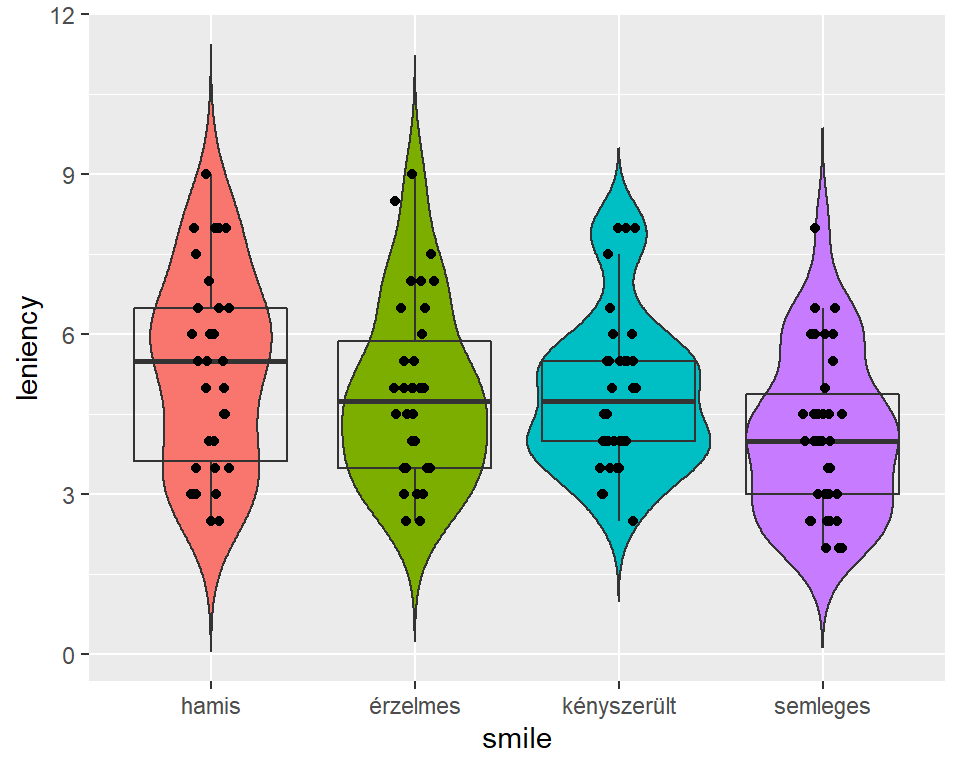
\includegraphics{02-peldak_files/figure-latex/unnamed-chunk-3-1} 

}

\caption{Dobozdiagram}\label{fig:unnamed-chunk-3}
\end{figure}

\begin{Shaded}
\begin{Highlighting}[]
\CommentTok{\# Hipotézisvizsgálat}
\NormalTok{leniency\_model }\OtherTok{\textless{}{-}} \FunctionTok{aov}\NormalTok{(leniency}\SpecialCharTok{\textasciitilde{}}\NormalTok{smile, }\AttributeTok{data =}\NormalTok{ leniency)}
\FunctionTok{summary}\NormalTok{(leniency\_model)}
\CommentTok{\#\textgreater{}              Df Sum Sq Mean Sq F value Pr(\textgreater{}F)  }
\CommentTok{\#\textgreater{} smile         3   27.5   9.178   3.465 0.0182 *}
\CommentTok{\#\textgreater{} Residuals   132  349.7   2.649                 }
\CommentTok{\#\textgreater{} {-}{-}{-}}
\CommentTok{\#\textgreater{} Signif. codes:  }
\CommentTok{\#\textgreater{} 0 \textquotesingle{}***\textquotesingle{} 0.001 \textquotesingle{}**\textquotesingle{} 0.01 \textquotesingle{}*\textquotesingle{} 0.05 \textquotesingle{}.\textquotesingle{} 0.1 \textquotesingle{} \textquotesingle{} 1}
\FunctionTok{TukeyHSD}\NormalTok{(leniency\_model)}
\CommentTok{\#\textgreater{}   Tukey multiple comparisons of means}
\CommentTok{\#\textgreater{}     95\% family{-}wise confidence level}
\CommentTok{\#\textgreater{} }
\CommentTok{\#\textgreater{} Fit: aov(formula = leniency \textasciitilde{} smile, data = leniency)}
\CommentTok{\#\textgreater{} }
\CommentTok{\#\textgreater{} $smile}
\CommentTok{\#\textgreater{}                            diff       lwr        upr}
\CommentTok{\#\textgreater{} érzelmes{-}hamis       {-}0.4558824 {-}1.483012  0.5712478}
\CommentTok{\#\textgreater{} kényszerült{-}hamis    {-}0.4558824 {-}1.483012  0.5712478}
\CommentTok{\#\textgreater{} semleges{-}hamis       {-}1.2500000 {-}2.277130 {-}0.2228699}
\CommentTok{\#\textgreater{} kényszerült{-}érzelmes  0.0000000 {-}1.027130  1.0271301}
\CommentTok{\#\textgreater{} semleges{-}érzelmes    {-}0.7941176 {-}1.821248  0.2330125}
\CommentTok{\#\textgreater{} semleges{-}kényszerült {-}0.7941176 {-}1.821248  0.2330125}
\CommentTok{\#\textgreater{}                          p adj}
\CommentTok{\#\textgreater{} érzelmes{-}hamis       0.6562329}
\CommentTok{\#\textgreater{} kényszerült{-}hamis    0.6562329}
\CommentTok{\#\textgreater{} semleges{-}hamis       0.0102192}
\CommentTok{\#\textgreater{} kényszerült{-}érzelmes 1.0000000}
\CommentTok{\#\textgreater{} semleges{-}érzelmes    0.1888804}
\CommentTok{\#\textgreater{} semleges{-}kényszerült 0.1888804}
\FunctionTok{library}\NormalTok{(DescTools)}
\FunctionTok{DunnettTest}\NormalTok{(leniency}\SpecialCharTok{\textasciitilde{}}\NormalTok{smile, }\AttributeTok{data =}\NormalTok{ leniency, }
            \AttributeTok{control =} \StringTok{"semleges"}\NormalTok{)}
\CommentTok{\#\textgreater{} }
\CommentTok{\#\textgreater{}   Dunnett\textquotesingle{}s test for comparing several treatments with a control :  }
\CommentTok{\#\textgreater{}     95\% family{-}wise confidence level}
\CommentTok{\#\textgreater{} }
\CommentTok{\#\textgreater{} $semleges}
\CommentTok{\#\textgreater{}                           diff     lwr.ci   upr.ci   pval}
\CommentTok{\#\textgreater{} hamis{-}semleges       1.2500000  0.3119186 2.188081 0.0055}
\CommentTok{\#\textgreater{} érzelmes{-}semleges    0.7941176 {-}0.1439637 1.732199 0.1162}
\CommentTok{\#\textgreater{} kényszerült{-}semleges 0.7941176 {-}0.1439637 1.732199 0.1164}
\CommentTok{\#\textgreater{}                         }
\CommentTok{\#\textgreater{} hamis{-}semleges       ** }
\CommentTok{\#\textgreater{} érzelmes{-}semleges       }
\CommentTok{\#\textgreater{} kényszerült{-}semleges    }
\CommentTok{\#\textgreater{} }
\CommentTok{\#\textgreater{} {-}{-}{-}}
\CommentTok{\#\textgreater{} Signif. codes:  0 \textquotesingle{}***\textquotesingle{} 0.001 \textquotesingle{}**\textquotesingle{} 0.01 \textquotesingle{}*\textquotesingle{} 0.05 \textquotesingle{}.\textquotesingle{} 0.1 \textquotesingle{} \textquotesingle{} 1}
\end{Highlighting}
\end{Shaded}

\hypertarget{jaspdata}{%
\section{JASPDATA}\label{jaspdata}}

\textbf{Hivatkozás a könyvre:}

Wagenmakers, E.-J., Kucharský, Š., \& the JASP Team. (2020). The JASP Data Library (1st ed.). \url{https://doi.org/10.6084/m9.figshare.9980744}

\href{https://jasp-stats.org/wp-content/uploads/2020/05/The_JASP_Data_Library_1st_Edition.pdf}{A könyv elérése}

\hypertarget{a-sleep-adatbuxe1zis}{%
\subsection{\texorpdfstring{A \texttt{sleep} adatbázis}{A sleep adatbázis}}\label{a-sleep-adatbuxe1zis}}

\hypertarget{leuxedruxe1s-1}{%
\subsubsection*{Leírás}\label{leuxedruxe1s-1}}
\addcontentsline{toc}{subsubsection}{Leírás}

Ez a híres ``Sleep'' (Alvás) adatmátrix, amelyet Student és Fisher is használt cikkeiben. A vizsgálatban 10 személy szerepelt, akik mindegyike 2 altatót is kapott két különböző időpontban. Az adatbázisban azokat a plusz órákat rögzítettük, amelyeket az egyes altatóknak köszönhetünk.

\hypertarget{vuxe1ltozuxf3k-1}{%
\subsubsection*{Változók}\label{vuxe1ltozuxf3k-1}}
\addcontentsline{toc}{subsubsection}{Változók}

\begin{itemize}
\tightlist
\item
  \texttt{extra} (numerikus) - Az extra órák száma az adott altató hatására a placebó altatóhoz képest.
\item
  \texttt{group} (faktor) - Az altató típusa. Lehetséges értéke: \texttt{1} és \texttt{2}.
\item
  \texttt{ID} (faktor) - A személy azonosítója.
\end{itemize}

Az adatbázisban a páros minta hosszú formában van eltárolva.

\hypertarget{hivatkozuxe1s-1}{%
\subsubsection*{Hivatkozás}\label{hivatkozuxe1s-1}}
\addcontentsline{toc}{subsubsection}{Hivatkozás}

\begin{itemize}
\tightlist
\item
  Cushny, A. R and Peebles, A. R. (1905). The action of optical isomers. The Journal of Physiology, 32: 501-510.
\item
  \href{https://jasp-stats.org/wp-content/uploads/2020/05/The_JASP_Data_Library_1st_Edition.pdf}{A könyvben a 21--27. oldalak}
\end{itemize}

\hypertarget{kapcsoluxf3duxf3-r-sorok-1}{%
\subsubsection*{Kapcsolódó R sorok}\label{kapcsoluxf3duxf3-r-sorok-1}}
\addcontentsline{toc}{subsubsection}{Kapcsolódó R sorok}

\begin{Shaded}
\begin{Highlighting}[]
\CommentTok{\# Beolvasás }
\NormalTok{sleep }\OtherTok{\textless{}{-}} \FunctionTok{read.table}\NormalTok{(}\AttributeTok{file =} \StringTok{"adat/jaspdata/sleep.csv"}\NormalTok{, }
                    \AttributeTok{sep =} \StringTok{","}\NormalTok{, }
                    \AttributeTok{dec =} \StringTok{"."}\NormalTok{,}
                    \AttributeTok{header =}\NormalTok{ T, }
                    \AttributeTok{quote =} \StringTok{""}\NormalTok{,  }
                    \AttributeTok{comment.char =} \StringTok{""}\NormalTok{, }
                    \AttributeTok{fileEncoding =} \StringTok{"UTF{-}8"}
\NormalTok{                    )}
\CommentTok{\# Típuskonverzió}
\NormalTok{sleep}\SpecialCharTok{$}\NormalTok{group }\OtherTok{\textless{}{-}} \FunctionTok{factor}\NormalTok{(sleep}\SpecialCharTok{$}\NormalTok{group)}
\NormalTok{sleep}\SpecialCharTok{$}\NormalTok{ID }\OtherTok{\textless{}{-}} \FunctionTok{factor}\NormalTok{(sleep}\SpecialCharTok{$}\NormalTok{ID)}
\FunctionTok{str}\NormalTok{(sleep)}
\CommentTok{\#\textgreater{} \textquotesingle{}data.frame\textquotesingle{}:    20 obs. of  3 variables:}
\CommentTok{\#\textgreater{}  $ extra: num  0.7 {-}1.6 {-}0.2 {-}1.2 {-}0.1 3.4 3.7 0.8 0 2 ...}
\CommentTok{\#\textgreater{}  $ group: Factor w/ 2 levels "1","2": 1 1 1 1 1 1 1 1 1 1 ...}
\CommentTok{\#\textgreater{}  $ ID   : Factor w/ 10 levels "1","2","3","4",..: 1 2 3 4 5 6 7 8 9 10 ...}

\CommentTok{\# Leíró statisztikai mutatók}
\FunctionTok{library}\NormalTok{(DescTools)}
\FunctionTok{Desc}\NormalTok{(}\AttributeTok{formula =}\NormalTok{ extra}\SpecialCharTok{\textasciitilde{}}\NormalTok{group, }\AttributeTok{data =}\NormalTok{ sleep, }\AttributeTok{plotit =}\NormalTok{ F)}
\CommentTok{\#\textgreater{} {-}{-}{-}{-}{-}{-}{-}{-}{-}{-}{-}{-}{-}{-}{-}{-}{-}{-}{-}{-}{-}{-}{-}{-}{-}{-}{-}{-}{-}{-}{-}{-}{-}{-}{-}{-}{-}{-}{-}{-}{-}{-}{-}{-}{-}{-}{-}{-}{-}{-}{-}{-}{-}{-}{-}{-}{-}{-} }
\CommentTok{\#\textgreater{} extra \textasciitilde{} group (sleep)}
\CommentTok{\#\textgreater{} }
\CommentTok{\#\textgreater{} Summary: }
\CommentTok{\#\textgreater{} n pairs: 20, valid: 20 (100.0\%), missings: 0 (0.0\%), groups: 2}
\CommentTok{\#\textgreater{} }
\CommentTok{\#\textgreater{}                         }
\CommentTok{\#\textgreater{}               1        2}
\CommentTok{\#\textgreater{} mean      0.750    2.330}
\CommentTok{\#\textgreater{} median    0.350    1.750}
\CommentTok{\#\textgreater{} sd        1.789    2.002}
\CommentTok{\#\textgreater{} IQR       1.875    3.275}
\CommentTok{\#\textgreater{} n            10       10}
\CommentTok{\#\textgreater{} np      50.000\%  50.000\%}
\CommentTok{\#\textgreater{} NAs           0        0}
\CommentTok{\#\textgreater{} 0s            1        0}
\CommentTok{\#\textgreater{} }
\CommentTok{\#\textgreater{} Kruskal{-}Wallis rank sum test:}
\CommentTok{\#\textgreater{}   Kruskal{-}Wallis chi{-}squared = 3.4378, df = 1, p{-}value = 0.06372}
\end{Highlighting}
\end{Shaded}

\begin{Shaded}
\begin{Highlighting}[]
\CommentTok{\# Leíró statisztikai mutatók}
\FunctionTok{library}\NormalTok{(psych)}
\NormalTok{temp }\OtherTok{\textless{}{-}} \FunctionTok{describeBy}\NormalTok{(}\AttributeTok{x =}\NormalTok{ extra}\SpecialCharTok{\textasciitilde{}}\NormalTok{group, }\AttributeTok{data =}\NormalTok{ sleep, }\AttributeTok{mat=}\NormalTok{T, }\AttributeTok{fast=}\NormalTok{T, }\AttributeTok{digits =} \DecValTok{2}\NormalTok{)}
\NormalTok{knitr}\SpecialCharTok{::}\FunctionTok{kable}\NormalTok{(temp, }\AttributeTok{caption =} \StringTok{"Leíró statisztikai mutatók"}\NormalTok{)}
\end{Highlighting}
\end{Shaded}

\begin{table}

\caption{\label{tab:unnamed-chunk-6}Leíró statisztikai mutatók}
\centering
\begin{tabular}[t]{l|l|l|r|r|r|r|r|r|r|r}
\hline
  & item & group1 & vars & n & mean & sd & min & max & range & se\\
\hline
X11 & 1 & 1 & 1 & 10 & 0.75 & 1.79 & -1.6 & 3.7 & 5.3 & 0.57\\
\hline
X12 & 2 & 2 & 1 & 10 & 2.33 & 2.00 & -0.1 & 5.5 & 5.6 & 0.63\\
\hline
\end{tabular}
\end{table}

\begin{Shaded}
\begin{Highlighting}[]

\FunctionTok{library}\NormalTok{(flextable)}
\FunctionTok{library}\NormalTok{(magrittr)}
\NormalTok{temp }\SpecialCharTok{\%\textgreater{}\%} \FunctionTok{flextable}\NormalTok{() }\SpecialCharTok{\%\textgreater{}\%} \FunctionTok{autofit}\NormalTok{()}
\end{Highlighting}
\end{Shaded}

\providecommand{\docline}[3]{\noalign{\global\setlength{\arrayrulewidth}{#1}}\arrayrulecolor[HTML]{#2}\cline{#3}}

\setlength{\tabcolsep}{2pt}

\renewcommand*{\arraystretch}{1.5}

\begin{longtable}[c]{|p{0.57in}|p{0.76in}|p{0.57in}|p{0.46in}|p{0.67in}|p{0.58in}|p{0.55in}|p{0.57in}|p{0.68in}|p{0.58in}}



\hhline{>{\arrayrulecolor[HTML]{666666}\global\arrayrulewidth=2pt}->{\arrayrulecolor[HTML]{666666}\global\arrayrulewidth=2pt}->{\arrayrulecolor[HTML]{666666}\global\arrayrulewidth=2pt}->{\arrayrulecolor[HTML]{666666}\global\arrayrulewidth=2pt}->{\arrayrulecolor[HTML]{666666}\global\arrayrulewidth=2pt}->{\arrayrulecolor[HTML]{666666}\global\arrayrulewidth=2pt}->{\arrayrulecolor[HTML]{666666}\global\arrayrulewidth=2pt}->{\arrayrulecolor[HTML]{666666}\global\arrayrulewidth=2pt}->{\arrayrulecolor[HTML]{666666}\global\arrayrulewidth=2pt}->{\arrayrulecolor[HTML]{666666}\global\arrayrulewidth=2pt}-}

\multicolumn{1}{!{\color[HTML]{000000}\vrule width 0pt}>{\raggedright}p{\dimexpr 0.57in+0\tabcolsep+0\arrayrulewidth}}{\fontsize{11}{11}\selectfont{\textcolor[HTML]{000000}{\global\setmainfont{Arial}item}}} & \multicolumn{1}{!{\color[HTML]{000000}\vrule width 0pt}>{\raggedright}p{\dimexpr 0.76in+0\tabcolsep+0\arrayrulewidth}}{\fontsize{11}{11}\selectfont{\textcolor[HTML]{000000}{\global\setmainfont{Arial}group1}}} & \multicolumn{1}{!{\color[HTML]{000000}\vrule width 0pt}>{\raggedleft}p{\dimexpr 0.57in+0\tabcolsep+0\arrayrulewidth}}{\fontsize{11}{11}\selectfont{\textcolor[HTML]{000000}{\global\setmainfont{Arial}vars}}} & \multicolumn{1}{!{\color[HTML]{000000}\vrule width 0pt}>{\raggedleft}p{\dimexpr 0.46in+0\tabcolsep+0\arrayrulewidth}}{\fontsize{11}{11}\selectfont{\textcolor[HTML]{000000}{\global\setmainfont{Arial}n}}} & \multicolumn{1}{!{\color[HTML]{000000}\vrule width 0pt}>{\raggedleft}p{\dimexpr 0.67in+0\tabcolsep+0\arrayrulewidth}}{\fontsize{11}{11}\selectfont{\textcolor[HTML]{000000}{\global\setmainfont{Arial}mean}}} & \multicolumn{1}{!{\color[HTML]{000000}\vrule width 0pt}>{\raggedleft}p{\dimexpr 0.58in+0\tabcolsep+0\arrayrulewidth}}{\fontsize{11}{11}\selectfont{\textcolor[HTML]{000000}{\global\setmainfont{Arial}sd}}} & \multicolumn{1}{!{\color[HTML]{000000}\vrule width 0pt}>{\raggedleft}p{\dimexpr 0.55in+0\tabcolsep+0\arrayrulewidth}}{\fontsize{11}{11}\selectfont{\textcolor[HTML]{000000}{\global\setmainfont{Arial}min}}} & \multicolumn{1}{!{\color[HTML]{000000}\vrule width 0pt}>{\raggedleft}p{\dimexpr 0.57in+0\tabcolsep+0\arrayrulewidth}}{\fontsize{11}{11}\selectfont{\textcolor[HTML]{000000}{\global\setmainfont{Arial}max}}} & \multicolumn{1}{!{\color[HTML]{000000}\vrule width 0pt}>{\raggedleft}p{\dimexpr 0.68in+0\tabcolsep+0\arrayrulewidth}}{\fontsize{11}{11}\selectfont{\textcolor[HTML]{000000}{\global\setmainfont{Arial}range}}} & \multicolumn{1}{!{\color[HTML]{000000}\vrule width 0pt}>{\raggedleft}p{\dimexpr 0.58in+0\tabcolsep+0\arrayrulewidth}!{\color[HTML]{000000}\vrule width 0pt}}{\fontsize{11}{11}\selectfont{\textcolor[HTML]{000000}{\global\setmainfont{Arial}se}}} \\

\noalign{\global\setlength{\arrayrulewidth}{2pt}}\arrayrulecolor[HTML]{666666}\cline{1-10}

\endfirsthead

\hhline{>{\arrayrulecolor[HTML]{666666}\global\arrayrulewidth=2pt}->{\arrayrulecolor[HTML]{666666}\global\arrayrulewidth=2pt}->{\arrayrulecolor[HTML]{666666}\global\arrayrulewidth=2pt}->{\arrayrulecolor[HTML]{666666}\global\arrayrulewidth=2pt}->{\arrayrulecolor[HTML]{666666}\global\arrayrulewidth=2pt}->{\arrayrulecolor[HTML]{666666}\global\arrayrulewidth=2pt}->{\arrayrulecolor[HTML]{666666}\global\arrayrulewidth=2pt}->{\arrayrulecolor[HTML]{666666}\global\arrayrulewidth=2pt}->{\arrayrulecolor[HTML]{666666}\global\arrayrulewidth=2pt}->{\arrayrulecolor[HTML]{666666}\global\arrayrulewidth=2pt}-}

\multicolumn{1}{!{\color[HTML]{000000}\vrule width 0pt}>{\raggedright}p{\dimexpr 0.57in+0\tabcolsep+0\arrayrulewidth}}{\fontsize{11}{11}\selectfont{\textcolor[HTML]{000000}{\global\setmainfont{Arial}item}}} & \multicolumn{1}{!{\color[HTML]{000000}\vrule width 0pt}>{\raggedright}p{\dimexpr 0.76in+0\tabcolsep+0\arrayrulewidth}}{\fontsize{11}{11}\selectfont{\textcolor[HTML]{000000}{\global\setmainfont{Arial}group1}}} & \multicolumn{1}{!{\color[HTML]{000000}\vrule width 0pt}>{\raggedleft}p{\dimexpr 0.57in+0\tabcolsep+0\arrayrulewidth}}{\fontsize{11}{11}\selectfont{\textcolor[HTML]{000000}{\global\setmainfont{Arial}vars}}} & \multicolumn{1}{!{\color[HTML]{000000}\vrule width 0pt}>{\raggedleft}p{\dimexpr 0.46in+0\tabcolsep+0\arrayrulewidth}}{\fontsize{11}{11}\selectfont{\textcolor[HTML]{000000}{\global\setmainfont{Arial}n}}} & \multicolumn{1}{!{\color[HTML]{000000}\vrule width 0pt}>{\raggedleft}p{\dimexpr 0.67in+0\tabcolsep+0\arrayrulewidth}}{\fontsize{11}{11}\selectfont{\textcolor[HTML]{000000}{\global\setmainfont{Arial}mean}}} & \multicolumn{1}{!{\color[HTML]{000000}\vrule width 0pt}>{\raggedleft}p{\dimexpr 0.58in+0\tabcolsep+0\arrayrulewidth}}{\fontsize{11}{11}\selectfont{\textcolor[HTML]{000000}{\global\setmainfont{Arial}sd}}} & \multicolumn{1}{!{\color[HTML]{000000}\vrule width 0pt}>{\raggedleft}p{\dimexpr 0.55in+0\tabcolsep+0\arrayrulewidth}}{\fontsize{11}{11}\selectfont{\textcolor[HTML]{000000}{\global\setmainfont{Arial}min}}} & \multicolumn{1}{!{\color[HTML]{000000}\vrule width 0pt}>{\raggedleft}p{\dimexpr 0.57in+0\tabcolsep+0\arrayrulewidth}}{\fontsize{11}{11}\selectfont{\textcolor[HTML]{000000}{\global\setmainfont{Arial}max}}} & \multicolumn{1}{!{\color[HTML]{000000}\vrule width 0pt}>{\raggedleft}p{\dimexpr 0.68in+0\tabcolsep+0\arrayrulewidth}}{\fontsize{11}{11}\selectfont{\textcolor[HTML]{000000}{\global\setmainfont{Arial}range}}} & \multicolumn{1}{!{\color[HTML]{000000}\vrule width 0pt}>{\raggedleft}p{\dimexpr 0.58in+0\tabcolsep+0\arrayrulewidth}!{\color[HTML]{000000}\vrule width 0pt}}{\fontsize{11}{11}\selectfont{\textcolor[HTML]{000000}{\global\setmainfont{Arial}se}}} \\

\noalign{\global\setlength{\arrayrulewidth}{2pt}}\arrayrulecolor[HTML]{666666}\cline{1-10}\endhead



\multicolumn{1}{!{\color[HTML]{000000}\vrule width 0pt}>{\raggedright}p{\dimexpr 0.57in+0\tabcolsep+0\arrayrulewidth}}{\fontsize{11}{11}\selectfont{\textcolor[HTML]{000000}{\global\setmainfont{Arial}1}}} & \multicolumn{1}{!{\color[HTML]{000000}\vrule width 0pt}>{\raggedright}p{\dimexpr 0.76in+0\tabcolsep+0\arrayrulewidth}}{\fontsize{11}{11}\selectfont{\textcolor[HTML]{000000}{\global\setmainfont{Arial}1}}} & \multicolumn{1}{!{\color[HTML]{000000}\vrule width 0pt}>{\raggedleft}p{\dimexpr 0.57in+0\tabcolsep+0\arrayrulewidth}}{\fontsize{11}{11}\selectfont{\textcolor[HTML]{000000}{\global\setmainfont{Arial}1}}} & \multicolumn{1}{!{\color[HTML]{000000}\vrule width 0pt}>{\raggedleft}p{\dimexpr 0.46in+0\tabcolsep+0\arrayrulewidth}}{\fontsize{11}{11}\selectfont{\textcolor[HTML]{000000}{\global\setmainfont{Arial}10}}} & \multicolumn{1}{!{\color[HTML]{000000}\vrule width 0pt}>{\raggedleft}p{\dimexpr 0.67in+0\tabcolsep+0\arrayrulewidth}}{\fontsize{11}{11}\selectfont{\textcolor[HTML]{000000}{\global\setmainfont{Arial}0.75}}} & \multicolumn{1}{!{\color[HTML]{000000}\vrule width 0pt}>{\raggedleft}p{\dimexpr 0.58in+0\tabcolsep+0\arrayrulewidth}}{\fontsize{11}{11}\selectfont{\textcolor[HTML]{000000}{\global\setmainfont{Arial}1.79}}} & \multicolumn{1}{!{\color[HTML]{000000}\vrule width 0pt}>{\raggedleft}p{\dimexpr 0.55in+0\tabcolsep+0\arrayrulewidth}}{\fontsize{11}{11}\selectfont{\textcolor[HTML]{000000}{\global\setmainfont{Arial}-1.6}}} & \multicolumn{1}{!{\color[HTML]{000000}\vrule width 0pt}>{\raggedleft}p{\dimexpr 0.57in+0\tabcolsep+0\arrayrulewidth}}{\fontsize{11}{11}\selectfont{\textcolor[HTML]{000000}{\global\setmainfont{Arial}3.7}}} & \multicolumn{1}{!{\color[HTML]{000000}\vrule width 0pt}>{\raggedleft}p{\dimexpr 0.68in+0\tabcolsep+0\arrayrulewidth}}{\fontsize{11}{11}\selectfont{\textcolor[HTML]{000000}{\global\setmainfont{Arial}5.3}}} & \multicolumn{1}{!{\color[HTML]{000000}\vrule width 0pt}>{\raggedleft}p{\dimexpr 0.58in+0\tabcolsep+0\arrayrulewidth}!{\color[HTML]{000000}\vrule width 0pt}}{\fontsize{11}{11}\selectfont{\textcolor[HTML]{000000}{\global\setmainfont{Arial}0.57}}} \\





\multicolumn{1}{!{\color[HTML]{000000}\vrule width 0pt}>{\raggedright}p{\dimexpr 0.57in+0\tabcolsep+0\arrayrulewidth}}{\fontsize{11}{11}\selectfont{\textcolor[HTML]{000000}{\global\setmainfont{Arial}2}}} & \multicolumn{1}{!{\color[HTML]{000000}\vrule width 0pt}>{\raggedright}p{\dimexpr 0.76in+0\tabcolsep+0\arrayrulewidth}}{\fontsize{11}{11}\selectfont{\textcolor[HTML]{000000}{\global\setmainfont{Arial}2}}} & \multicolumn{1}{!{\color[HTML]{000000}\vrule width 0pt}>{\raggedleft}p{\dimexpr 0.57in+0\tabcolsep+0\arrayrulewidth}}{\fontsize{11}{11}\selectfont{\textcolor[HTML]{000000}{\global\setmainfont{Arial}1}}} & \multicolumn{1}{!{\color[HTML]{000000}\vrule width 0pt}>{\raggedleft}p{\dimexpr 0.46in+0\tabcolsep+0\arrayrulewidth}}{\fontsize{11}{11}\selectfont{\textcolor[HTML]{000000}{\global\setmainfont{Arial}10}}} & \multicolumn{1}{!{\color[HTML]{000000}\vrule width 0pt}>{\raggedleft}p{\dimexpr 0.67in+0\tabcolsep+0\arrayrulewidth}}{\fontsize{11}{11}\selectfont{\textcolor[HTML]{000000}{\global\setmainfont{Arial}2.33}}} & \multicolumn{1}{!{\color[HTML]{000000}\vrule width 0pt}>{\raggedleft}p{\dimexpr 0.58in+0\tabcolsep+0\arrayrulewidth}}{\fontsize{11}{11}\selectfont{\textcolor[HTML]{000000}{\global\setmainfont{Arial}2.00}}} & \multicolumn{1}{!{\color[HTML]{000000}\vrule width 0pt}>{\raggedleft}p{\dimexpr 0.55in+0\tabcolsep+0\arrayrulewidth}}{\fontsize{11}{11}\selectfont{\textcolor[HTML]{000000}{\global\setmainfont{Arial}-0.1}}} & \multicolumn{1}{!{\color[HTML]{000000}\vrule width 0pt}>{\raggedleft}p{\dimexpr 0.57in+0\tabcolsep+0\arrayrulewidth}}{\fontsize{11}{11}\selectfont{\textcolor[HTML]{000000}{\global\setmainfont{Arial}5.5}}} & \multicolumn{1}{!{\color[HTML]{000000}\vrule width 0pt}>{\raggedleft}p{\dimexpr 0.68in+0\tabcolsep+0\arrayrulewidth}}{\fontsize{11}{11}\selectfont{\textcolor[HTML]{000000}{\global\setmainfont{Arial}5.6}}} & \multicolumn{1}{!{\color[HTML]{000000}\vrule width 0pt}>{\raggedleft}p{\dimexpr 0.58in+0\tabcolsep+0\arrayrulewidth}!{\color[HTML]{000000}\vrule width 0pt}}{\fontsize{11}{11}\selectfont{\textcolor[HTML]{000000}{\global\setmainfont{Arial}0.63}}} \\

\noalign{\global\setlength{\arrayrulewidth}{2pt}}\arrayrulecolor[HTML]{666666}\cline{1-10}

\end{longtable}

\begin{Shaded}
\begin{Highlighting}[]
\CommentTok{\# Leíró statisztikai mutatók}
\FunctionTok{library}\NormalTok{(summarytools)}
\FunctionTok{st\_options}\NormalTok{(}\StringTok{"headings"}\NormalTok{, }\ConstantTok{FALSE}\NormalTok{)}
\FunctionTok{with}\NormalTok{(sleep, }
           \FunctionTok{stby}\NormalTok{(}\AttributeTok{data =}\NormalTok{ extra, }
                \AttributeTok{INDICES =}\NormalTok{ group, }
                \AttributeTok{FUN =}\NormalTok{ descr,}
                \AttributeTok{stats =} \FunctionTok{c}\NormalTok{(}\StringTok{"n.valid"}\NormalTok{, }\StringTok{"mean"}\NormalTok{, }\StringTok{"sd"}\NormalTok{, }
                          \StringTok{"min"}\NormalTok{, }\StringTok{"med"}\NormalTok{, }\StringTok{"max"}\NormalTok{),}
                \AttributeTok{transpose =} \ConstantTok{FALSE}\NormalTok{,}
                \AttributeTok{style=}\StringTok{"rmarkdown"}\NormalTok{,}
                \AttributeTok{caption=}\StringTok{"Leíró statisztika"}
\NormalTok{                )) }
\end{Highlighting}
\end{Shaded}

\begin{longtable}[]{@{}lrr@{}}
\caption{Leíró statisztika}\tabularnewline
\toprule
& 1 & 2 \\
\midrule
\endfirsthead
\toprule
& 1 & 2 \\
\midrule
\endhead
N.Valid & 10.00 & 10.00 \\
Mean & 0.75 & 2.33 \\
Std.Dev & 1.79 & 2.00 \\
Min & -1.60 & -0.10 \\
Median & 0.35 & 1.75 \\
Max & 3.70 & 5.50 \\
\bottomrule
\end{longtable}

\begin{Shaded}
\begin{Highlighting}[]
\CommentTok{\# Ábra}
\FunctionTok{library}\NormalTok{(ggplot2)}
\FunctionTok{ggplot}\NormalTok{(}\AttributeTok{data =}\NormalTok{ sleep, }\AttributeTok{mapping =} \FunctionTok{aes}\NormalTok{(}\AttributeTok{x=}\NormalTok{group, }\AttributeTok{y=}\NormalTok{extra, }\AttributeTok{fill=}\NormalTok{group)) }\SpecialCharTok{+} 
  \FunctionTok{geom\_violin}\NormalTok{(}\AttributeTok{trim =} \ConstantTok{FALSE}\NormalTok{) }\SpecialCharTok{+} 
  \FunctionTok{geom\_boxplot}\NormalTok{(}\AttributeTok{alpha=}\DecValTok{0}\NormalTok{) }\SpecialCharTok{+} 
  \FunctionTok{geom\_jitter}\NormalTok{(}\AttributeTok{height =} \DecValTok{0}\NormalTok{, }\AttributeTok{width =} \FloatTok{0.1}\NormalTok{) }\SpecialCharTok{+} 
  \FunctionTok{theme}\NormalTok{(}\AttributeTok{legend.position =} \StringTok{"none"}\NormalTok{) }
\end{Highlighting}
\end{Shaded}

\begin{figure}

{\centering 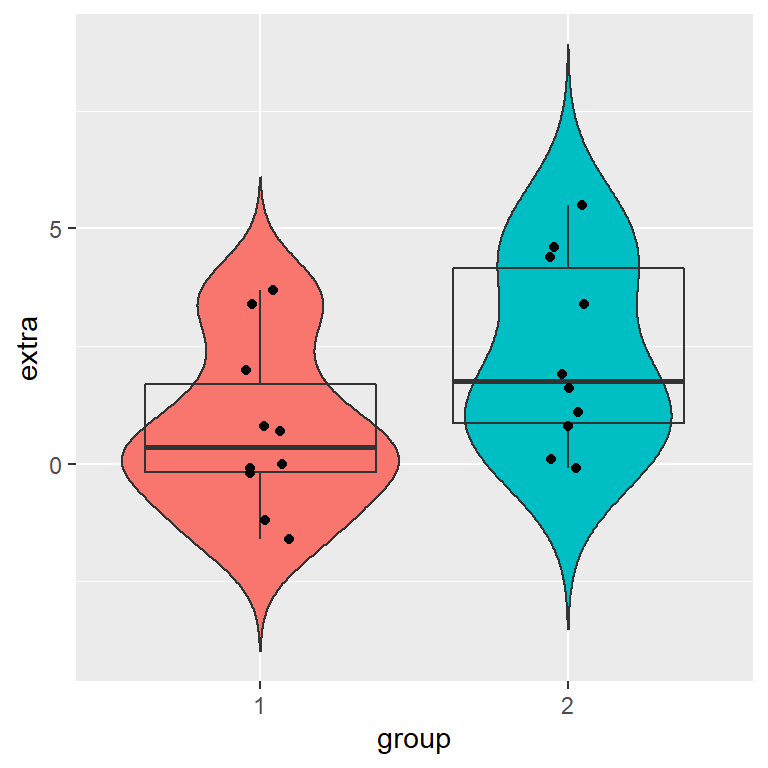
\includegraphics{02-peldak_files/figure-latex/unnamed-chunk-8-1} 

}

\caption{Dobozdiagram}\label{fig:unnamed-chunk-8}
\end{figure}

\begin{Shaded}
\begin{Highlighting}[]
\CommentTok{\# Ábra}
\FunctionTok{library}\NormalTok{(ggplot2)}
\FunctionTok{ggplot}\NormalTok{(}\AttributeTok{data =}\NormalTok{ sleep, }\AttributeTok{mapping =} \FunctionTok{aes}\NormalTok{(}\AttributeTok{x=}\NormalTok{group, }\AttributeTok{y=}\NormalTok{extra, }\AttributeTok{fill=}\NormalTok{group)) }\SpecialCharTok{+} 
  \FunctionTok{geom\_boxplot}\NormalTok{() }\SpecialCharTok{+} 
  \FunctionTok{geom\_line}\NormalTok{(}\FunctionTok{aes}\NormalTok{(}\AttributeTok{group=}\NormalTok{ID), }\AttributeTok{alpha=}\FloatTok{0.7}\NormalTok{) }\SpecialCharTok{+}  
  \FunctionTok{geom\_point}\NormalTok{() }\SpecialCharTok{+} 
  \FunctionTok{theme}\NormalTok{(}\AttributeTok{legend.position =} \StringTok{"none"}\NormalTok{) }
\end{Highlighting}
\end{Shaded}

\begin{figure}

{\centering 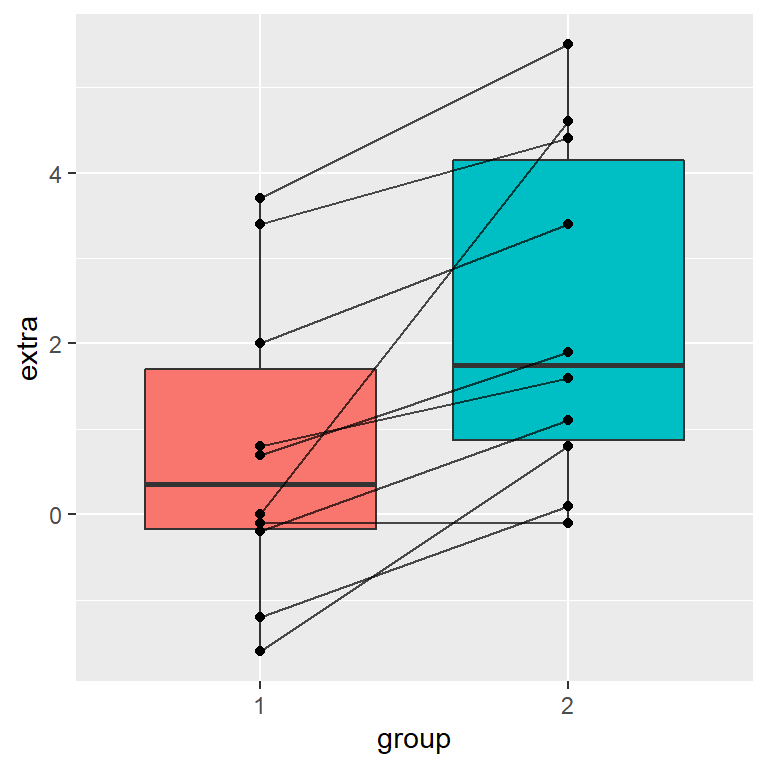
\includegraphics{02-peldak_files/figure-latex/unnamed-chunk-9-1} 

}

\caption{Dobozdiagram}\label{fig:unnamed-chunk-9}
\end{figure}

\begin{Shaded}
\begin{Highlighting}[]
\CommentTok{\# Hipotézisvizsgálat}
\FunctionTok{library}\NormalTok{(lsr)}
\FunctionTok{pairedSamplesTTest}\NormalTok{(}\AttributeTok{formula =}\NormalTok{ extra}\SpecialCharTok{\textasciitilde{}}\NormalTok{group, }\AttributeTok{data =}\NormalTok{ sleep, }\AttributeTok{id =} \StringTok{"ID"}\NormalTok{)}
\CommentTok{\#\textgreater{} }
\CommentTok{\#\textgreater{}    Paired samples t{-}test }
\CommentTok{\#\textgreater{} }
\CommentTok{\#\textgreater{} Outcome variable:   extra }
\CommentTok{\#\textgreater{} Grouping variable:  group }
\CommentTok{\#\textgreater{} ID variable:        ID }
\CommentTok{\#\textgreater{} }
\CommentTok{\#\textgreater{} Descriptive statistics: }
\CommentTok{\#\textgreater{}                 1     2 difference}
\CommentTok{\#\textgreater{}    mean     0.750 2.330     {-}1.580}
\CommentTok{\#\textgreater{}    std dev. 1.789 2.002      1.230}
\CommentTok{\#\textgreater{} }
\CommentTok{\#\textgreater{} Hypotheses: }
\CommentTok{\#\textgreater{}    null:        population means equal for both measurements}
\CommentTok{\#\textgreater{}    alternative: different population means for each measurement}
\CommentTok{\#\textgreater{} }
\CommentTok{\#\textgreater{} Test results: }
\CommentTok{\#\textgreater{}    t{-}statistic:  {-}4.062 }
\CommentTok{\#\textgreater{}    degrees of freedom:  9 }
\CommentTok{\#\textgreater{}    p{-}value:  0.003 }
\CommentTok{\#\textgreater{} }
\CommentTok{\#\textgreater{} Other information: }
\CommentTok{\#\textgreater{}    two{-}sided 95\% confidence interval:  [{-}2.46, {-}0.7] }
\CommentTok{\#\textgreater{}    estimated effect size (Cohen\textquotesingle{}s d):  1.285}
\end{Highlighting}
\end{Shaded}


  \bibliography{book.bib,packages.bib}

\end{document}
